% Lecture 2 --- Brownian motion, stopping times, and roughness
\documentclass[10pt,aspectratio=169]{beamer}

\usepackage[utf8]{inputenc}
\usepackage[T1]{fontenc}
\usepackage[english]{babel}
\usepackage{lmodern}
\usepackage{microtype}
\usepackage{amsmath,amssymb,bm,mathtools}
\usepackage{booktabs}
\usepackage{graphicx}
\usepackage{tikz}
\usetikzlibrary{arrows.meta,positioning,calc}

\usetheme[numbering=fraction,progressbar=frametitle]{metropolis}
\setbeamertemplate{frame numbering}[fraction]
\setbeamertemplate{navigation symbols}{}

\definecolor{BootcampBlueDark}{HTML}{1A3C68}
\definecolor{BootcampBlue}{RGB}{31,110,178}
\definecolor{AccentGold}{HTML}{DAA520}
\definecolor{SoftGray}{RGB}{245,246,248}
\definecolor{TextBlack}{HTML}{000000}
\definecolor{Crimson}{HTML}{990000}
\definecolor{MatrixGreen}{HTML}{228B22}
\definecolor{MatrixRed}{HTML}{B22222}

\setbeamercolor{normal text}{fg=TextBlack,bg=white}
\setbeamercolor{title}{fg=TextBlack}
\setbeamerfont{title}{size=\Large,series=\bfseries}
\setbeamercolor{structure}{fg=BootcampBlueDark}
\setbeamercolor{progress bar}{fg=BootcampBlueDark,bg=gray!30}
\setbeamercolor{frametitle}{bg=BootcampBlueDark,fg=white}
\setbeamerfont{frametitle}{series=\bfseries,size=\large}
\setbeamertemplate{frametitle}{
  \nointerlineskip
  \begin{beamercolorbox}[wd=\paperwidth,ht=3.2ex,dp=1.4ex,leftskip=1em,rightskip=1em]{frametitle}
    \usebeamerfont{frametitle}\insertframetitle
  \end{beamercolorbox}
}

\setbeamercolor{block title example}{bg=BootcampBlueDark!90!black,fg=white}
\setbeamercolor{block body example}{bg=BootcampBlueDark!5!white,fg=black}
\setbeamercolor{block title proposition}{bg=MatrixGreen!75!black,fg=white}
\setbeamercolor{block body proposition}{bg=MatrixGreen!7!white,fg=black}
\setbeamertemplate{blocks}[rounded][shadow=false]

\newenvironment{definitionblock}[1]{%
  \par\vspace{0.35em}%
  \begin{beamercolorbox}[wd=\textwidth,sep=0.35em,leftskip=0.3em,rightskip=0.6em]{block title example}%
    \raisebox{0.12em}{\usebeamerfont{block title example}#1}%
  \end{beamercolorbox}%
  \vspace{-0.35em}%
  \begin{beamercolorbox}[wd=\textwidth,sep=0.75em,leftskip=0.6em,rightskip=0.6em]{block body example}%
    \usebeamerfont{block body example}%
}{%
  \end{beamercolorbox}%
  \par\vspace{0.45em}%
}

\newenvironment{propositionblock}[1]{%
  \par\vspace{0.35em}%
  \begin{beamercolorbox}[wd=\textwidth,sep=0.35em,leftskip=0.3em,rightskip=0.6em]{block title proposition}%
    \raisebox{0.12em}{\usebeamerfont{block title example}#1}%
  \end{beamercolorbox}%
  \vspace{-0.35em}%
  \begin{beamercolorbox}[wd=\textwidth,sep=0.75em,leftskip=0.6em,rightskip=0.6em]{block body proposition}%
    \usebeamerfont{block body example}%
}{%
  \end{beamercolorbox}%
  \par\vspace{0.45em}%
}

\newcommand{\E}{\mathbb E}
\newcommand{\Pp}{\mathbb P}
\newcommand{\F}{\mathcal F}
\newcommand{\R}{\mathbb R}

% One transition page per major section.
\AtBeginSection[]{
  \begin{frame}[plain]
    \vfill
    {\Large\bfseries\color{BootcampBlueDark}\insertsectionhead\par}
    \medskip
    {\color{BootcampBlueDark}\rule{0.9\textwidth}{0.8pt}}
    \vfill
  \end{frame}
}

\title{Brownian Motion, Stopping Times, and Quadratic Variation}
\author{}
\date{}

\begin{document}

\begin{frame}[plain]
  \vfill
  {\usebeamerfont{title}\usebeamercolor[fg]{title}\inserttitle\par}
  \medskip
  {\color{BootcampBlueDark}\rule{0.95\textwidth}{0.8pt}}
  \vfill
\end{frame}

\begin{frame}{References}
\footnotesize
\textbf{Main references}
\begin{itemize}\setlength{\itemsep}{0.5em}
  \item S.~Shreve, \emph{Stochastic Calculus for Finance II}, Chapter 3.
  \item I.~Karatzas and S.~Shreve, \emph{Brownian Motion and Stochastic Calculus}, Chapter 2.
  \item T.~Bj\"ork, \emph{Arbitrage Theory in Continuous Time}, chapters on Brownian motion and stochastic integration.
\end{itemize}
\end{frame}

\begin{frame}{Roadmap}
\begin{enumerate}\setlength{\itemsep}{0.45em}
  \item Define continuous-time stochastic processes and filtrations.
  \item Construct Brownian motion and identify its Gaussian structure.
  \item Read the weak Markov property as renewal at deterministic times.
  \item Introduce stopping times, \(\F_\tau\), and strong Markov renewal.
  \item Organize the reflection principle as a path transformation.
  \item Measure path roughness through quadratic variation.
  \item Turn Brownian motion into a positive price model.
\end{enumerate}
\end{frame}

% =====================================================
\section{Continuous-Time Stochastic Processes}
\subsection{Processes, paths, and information}

\begin{frame}{A stochastic process is a time-indexed family of random variables}
Let \((\Omega,\F,\Pp)\) be a probability space and let \(E\) be a state space.
\begin{definitionblock}{Stochastic process}
A continuous-time stochastic process is a family
\[
X=(X_t)_{t\ge0},
\qquad X_t:\Omega\to E,
\]
such that each \(X_t\) is a random variable.
\end{definitionblock}
\begin{columns}[T,onlytextwidth]
\column{0.48\textwidth}
\textbf{Time parameter}
\begin{itemize}
  \item discrete: \(t\in\{0,1,2,\ldots\}\);
  \item continuous: \(t\in[0,\infty)\).
\end{itemize}
\column{0.48\textwidth}
\textbf{Typical state spaces}
\begin{itemize}
  \item \(E=\R\): price or factor;
  \item \(E=\R^d\): several risk factors;
  \item \(E=\mathbb N\): event count.
\end{itemize}
\end{columns}
\end{frame}

\begin{frame}{One process has both distributional and pathwise descriptions}
For \(X:[0,\infty)\times\Omega\to E\), we can freeze either argument.
\begin{columns}[T,onlytextwidth]
\column{0.48\textwidth}
\begin{definitionblock}{Random variable at time \(t\)}
Fix \(t\). Then \(X_t:\omega\mapsto X_t(\omega)\) describes uncertainty across scenarios at that date.
\end{definitionblock}
The joint laws
\[
(X_{t_1},\ldots,X_{t_n})
\]
are the finite-dimensional distributions.
\column{0.48\textwidth}
\begin{definitionblock}{Sample path in scenario \(\omega\)}
Fix \(\omega\). Then
\[
t\longmapsto X_t(\omega)
\]
is one realized trajectory through time.
\end{definitionblock}
Path-dependent claims depend on the whole trajectory, not only on \(X_T\).
\end{columns}
\begin{block}{Important}
Marginal laws alone do not determine a process: dependence across dates matters.
\end{block}
\end{frame}

\begin{frame}{Path regularity and increments distinguish continuous-time models}
\begin{columns}[T,onlytextwidth]
\column{0.49\textwidth}
\begin{definitionblock}{Continuous paths}
The process has continuous paths if
\[
\Pp\bigl(t\mapsto X_t\text{ is continuous}\bigr)=1.
\]
\end{definitionblock}
\begin{definitionblock}{C\`adl\`ag paths}
Paths are right-continuous and have left limits. This allows jumps while ruling out pathological oscillations.
\end{definitionblock}
\column{0.47\textwidth}
For \(0\le s<t\), the increment is
\[
X_t-X_s.
\]
\begin{itemize}
  \item \textbf{stationary increments:} its law depends only on \(t-s\);
  \item \textbf{independent increments:} increments over disjoint intervals are independent.
\end{itemize}
Brownian motion has continuous paths and both increment properties.
\end{columns}
\end{frame}

\begin{frame}{A filtration records how information grows through time}
\begin{definitionblock}{Filtration}
A filtration \((\F_t)_{t\ge0}\) is an increasing family of sigma-fields:
\[
\F_s\subseteq\F_t\subseteq\F,
\qquad 0\le s\le t.
\]
The sigma-field \(\F_t\) represents everything observable by time \(t\).
\end{definitionblock}
\begin{definitionblock}{Natural filtration of a process}
\[
\F_t^X=\sigma(X_u:0\le u\le t).
\]
It contains exactly the information revealed by the path of \(X\) up to time \(t\).
\end{definitionblock}
In continuous time, one usually augments this filtration by null events and imposes right-continuity; these are the \emph{usual conditions}.
\end{frame}

\begin{frame}{Adaptedness prevents information from arriving from the future}
\begin{definitionblock}{Adapted process}
A process \(X\) is adapted to \((\F_t)\) if \(X_t\) is \(\F_t\)-measurable for every \(t\ge0\).
\end{definitionblock}
At time \(t\), an adapted quantity can be computed from currently available information.
\begin{columns}[T,onlytextwidth]
\column{0.48\textwidth}
\begin{block}{Admissible}
With \(\F_t^W=\sigma(W_u:u\le t)\), both \(W_t\) and
\(\max_{0\le u\le t}W_u\) are \(\F_t^W\)-measurable.
\end{block}
\column{0.48\textwidth}
\begin{block}{Not observable yet}
For \(h>0\), neither \(W_{t+h}\) nor the sign of \(W_{t+h}-W_t\) is known at time \(t\).
\end{block}
\end{columns}
In finance, a trading decision must be adapted -- and, for stochastic integration, typically predictable.
\end{frame}

\begin{frame}{Three conditional notions organize the rest of the lecture}
For an adapted process \(X\) and \(0\le s<t\):
\begin{description}\setlength{\itemsep}{0.65em}
  \item[Martingale:] if \(X_t\) is integrable and
  \[
  \E[X_t\mid\F_s]=X_s,
  \]
  the current value is the best conditional mean forecast.
  \item[Markov process:] the conditional law of the future given \(\F_s\) depends on the past only through the present state \(X_s\).
  \item[Stopping time:] a random time \(\tau\) satisfies
  \[
  \{\tau\le t\}\in\F_t;
  \]
  whether stopping has occurred is observable without looking ahead.
\end{description}
Brownian motion provides the canonical example of all three ideas.
\end{frame}

% =====================================================
\section{Brownian Construction and Gaussian Structure}
\subsection{Why Brownian motion?}

\begin{frame}{A useful continuous-time model must keep randomness and roughness}
\begin{columns}[T,onlytextwidth]
\column{0.55\textwidth}
Financial prices receive many small shocks:
\begin{itemize}
  \item information arrives through time;
  \item the direction of the next move is uncertain;
  \item paths look continuous at a daily scale but irregular when we zoom in.
\end{itemize}

\column{0.41\textwidth}
\centering
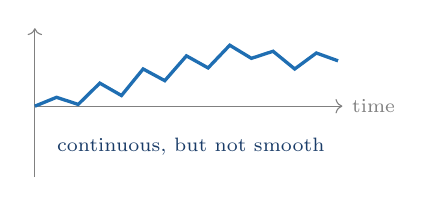
\begin{tikzpicture}[x=0.55cm,y=0.45cm]
  \draw[->,gray] (0,0) -- (7.1,0) node[right] {\scriptsize time};
  \draw[->,gray] (0,-2) -- (0,2.2);
  \draw[very thick,BootcampBlue]
    plot coordinates {(0,0) (.5,.25) (1,.05) (1.5,.65) (2,.3)
    (2.5,1.05) (3,.72) (3.5,1.42) (4,1.08) (4.5,1.72)
    (5,1.35) (5.5,1.55) (6,1.05) (6.5,1.5) (7,1.28)};
  \node[BootcampBlueDark] at (3.6,-1.15) {\scriptsize continuous, but not smooth};
\end{tikzpicture}
\end{columns}
\begin{block}{Modeling goal}
Construct a continuous process whose increments remain random at every time scale.
\end{block}
\end{frame}

\subsection{The discrete starting point}

\begin{frame}{The simple random walk accumulates independent shocks}
Let \(\varepsilon_1,\varepsilon_2,\ldots\) be i.i.d. with
\[
\Pp(\varepsilon_k=1)=\Pp(\varepsilon_k=-1)=\tfrac12,
\qquad
S_n=\sum_{k=1}^{n}\varepsilon_k.
\]
\begin{columns}[T,onlytextwidth]
\column{0.48\textwidth}
\begin{itemize}
  \item \(S_n\) is the position after \(n\) steps.
  \item \(\E[S_n]=0\) and \(\operatorname{Var}(S_n)=n\).
  \item A typical displacement therefore has size \(\sqrt n\).
\end{itemize}
\column{0.48\textwidth}
\centering
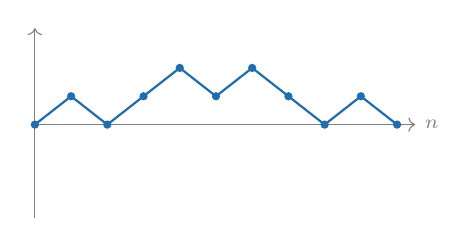
\begin{tikzpicture}[x=0.46cm,y=0.36cm]
  \draw[->,gray] (0,0) -- (10.5,0) node[right] {\scriptsize \(n\)};
  \draw[->,gray] (0,-3.3) -- (0,3.4);
  \draw[thick,BootcampBlue] plot coordinates
   {(0,0)(1,1)(2,0)(3,1)(4,2)(5,1)(6,2)(7,1)(8,0)(9,1)(10,0)};
  \foreach \x/\y in {0/0,1/1,2/0,3/1,4/2,5/1,6/2,7/1,8/0,9/1,10/0}
    \fill[BootcampBlue] (\x,\y) circle (1.5pt);
\end{tikzpicture}
\end{columns}
\end{frame}

\begin{frame}{Rescaling balances more steps with smaller shocks}
To fit \(n\) shocks into one unit of time, shrink each shock by \(1/\sqrt n\):
\[
W_t^{(n)}=\frac{S_{\lfloor nt\rfloor}}{\sqrt n},
\qquad 0\le t\le1,
\]
with linear interpolation between grid points.
\begin{center}
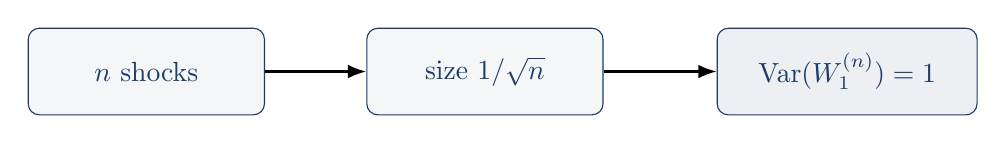
\begin{tikzpicture}[>=Latex]
  \node[draw,BootcampBlueDark,rounded corners,fill=SoftGray,
        minimum width=3cm,minimum height=1.1cm] (a) at (0,0) {\(n\) shocks};
  \node[draw,BootcampBlueDark,rounded corners,fill=SoftGray,
        minimum width=3cm,minimum height=1.1cm] (b) at (4.3,0) {size \(1/\sqrt n\)};
  \node[draw,BootcampBlueDark,rounded corners,fill=BootcampBlueDark!8,
        minimum width=3.3cm,minimum height=1.1cm] (c) at (8.9,0)
        {\(\operatorname{Var}(W_1^{(n)})=1\)};
  \draw[->,thick] (a) -- (b);
  \draw[->,thick] (b) -- (c);
\end{tikzpicture}
\end{center}
\begin{block}{Why \(1/\sqrt n\)?}
The total variance remains of order one: \(n\times(1/\sqrt n)^2=1\).
\end{block}
\end{frame}

\begin{frame}{Donsker explains why Brownian motion is the natural limit}
\begin{columns}[T,onlytextwidth]
\column{0.45\textwidth}
\centering
\textbf{Rescaled random walk}
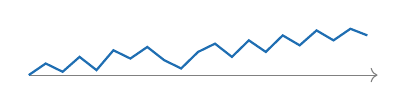
\begin{tikzpicture}[x=0.43cm,y=0.42cm]
  \draw[->,gray] (0,0) -- (10.3,0);
  \draw[thick,BootcampBlue] plot coordinates
    {(0,0)(.5,.35)(1,.1)(1.5,.55)(2,.15)(2.5,.75)(3,.5)
    (3.5,.85)(4,.45)(4.5,.2)(5,.7)(5.5,.95)(6,.55)(6.5,1.05)
    (7,.7)(7.5,1.2)(8,.9)(8.5,1.35)(9,1.05)(9.5,1.4)(10,1.2)};
\end{tikzpicture}
\column{0.06\textwidth}
\centering\vspace{1.2cm}\(\Longrightarrow\)
\column{0.45\textwidth}
\centering
\textbf{Brownian path}
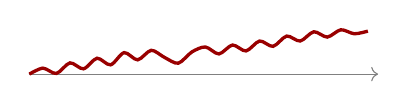
\begin{tikzpicture}[x=0.43cm,y=0.42cm]
  \draw[->,gray] (0,0) -- (10.3,0);
  \draw[very thick,Crimson,smooth] plot coordinates
    {(0,0)(.4,.18)(.8,.02)(1.2,.34)(1.6,.16)(2,.48)(2.4,.28)
    (2.8,.65)(3.2,.43)(3.6,.72)(4,.5)(4.4,.33)(4.8,.67)(5.2,.82)
    (5.6,.61)(6,.88)(6.4,.7)(6.8,1)(7.2,.84)(7.6,1.15)
    (8,1)(8.4,1.28)(8.8,1.12)(9.2,1.34)(9.6,1.22)(10,1.3)};
\end{tikzpicture}
\end{columns}
\begin{definitionblock}{Donsker's invariance principle, informal}
As the mesh goes to zero, the rescaled random-walk path \(W^{(n)}\) converges in distribution to a standard Brownian motion \(W\).
\end{definitionblock}
The theorem motivates the model; its technical proof is not needed for what follows.
\end{frame}

\subsection{The defining properties}

\begin{frame}{Four properties define standard Brownian motion}
\begin{definitionblock}{Standard Brownian motion}
A process \((W_t)_{t\ge0}\) is a standard Brownian motion if:
\begin{enumerate}
  \item \(W_0=0\);
  \item increments over disjoint time intervals are independent;
  \item \(W_t-W_s\sim\mathcal N(0,t-s)\) for \(0\le s<t\);
  \item \(t\mapsto W_t\) is continuous almost surely.
\end{enumerate}
\end{definitionblock}
\begin{block}{One-line interpretation}
Fresh shocks arrive independently, their scale depends only on elapsed time, and their accumulation produces a continuous but rough path.
\end{block}
\end{frame}

\begin{frame}{Independent increments mean that non-overlapping shocks are unrelated}
\begin{center}
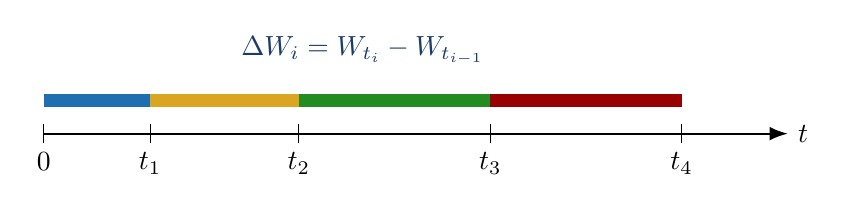
\begin{tikzpicture}[x=1.35cm,y=1cm,>=Latex]
  \draw[->,thick] (0,0) -- (7,0) node[right] {\(t\)};
  \foreach \x/\lab in {0/0,1/t_1,2.4/t_2,4.2/t_3,6/t_4}
    {\draw (\x,.12)--(\x,-.12) node[below] {\(\lab\)};}
  \draw[line width=5pt,BootcampBlue] (0,.42)--(1,.42);
  \draw[line width=5pt,AccentGold] (1,.42)--(2.4,.42);
  \draw[line width=5pt,MatrixGreen] (2.4,.42)--(4.2,.42);
  \draw[line width=5pt,Crimson] (4.2,.42)--(6,.42);
  \node[BootcampBlueDark] at (3,1.05) {\(\Delta W_i=W_{t_i}-W_{t_{i-1}}\)};
\end{tikzpicture}
\end{center}
For \(0=t_0<t_1<\cdots<t_m\), the increments
\[
W_{t_1}-W_{t_0},\ldots,W_{t_m}-W_{t_{m-1}}
\]
are independent.
\begin{block}{Concrete meaning}
Knowing that the path rose between \(t_1\) and \(t_2\) does not change the distribution of its move between \(t_3\) and \(t_4\).
\end{block}
\end{frame}

\begin{frame}{Stationary Gaussian increments turn elapsed time into uncertainty}
For every \(0\le s<t\),
\[
W_t-W_s\sim\mathcal N(0,t-s).
\]
\begin{columns}[T,onlytextwidth]
\column{0.47\textwidth}
\begin{definitionblock}{Stationary increments}
The law depends on the duration \(t-s\), not on the calendar location \(s\).
\end{definitionblock}
\[
W_{1.5}-W_{0.5}\ \overset{d}=\
W_{11}-W_{10}\sim\mathcal N(0,1).
\]
\column{0.47\textwidth}
\begin{definitionblock}{Gaussian increments}
Every increment is normally distributed, centered, and symmetric.
\end{definitionblock}
\[
\operatorname{SD}(W_t-W_s)=\sqrt{t-s}.
\]
\end{columns}
A four-times-longer interval produces twice the typical displacement.
\end{frame}

\begin{frame}{Small examples: use the four Brownian properties immediately}
Let \((W_t)_{t\ge0}\) be a standard Brownian motion with its natural filtration.
\begin{enumerate}\setlength{\itemsep}{0.75em}
  \item Since only elapsed time matters,
  \[
  W_4-W_1\sim\mathcal N(0,3).
  \]
  \item Since \(W_1\in\F_2\) and \(W_4-W_2\) is independent of \(\F_2\),
  \[
  \operatorname{Cov}(W_1,W_4-W_2)=0.
  \]
  \item By symmetry of every fresh Gaussian increment, for \(h>0\),
  \[
  \Pp(W_{t+h}>W_t\mid\F_t)=\tfrac12.
  \]
\end{enumerate}
Each calculation uses a different ingredient: stationarity, independence, or Gaussian symmetry.
\end{frame}

\begin{frame}{Quick diagnostic: which transformations are Brownian motions?}
Starting from a standard Brownian motion \(W\), consider
\[
X_t=-W_t,
\qquad
Y_t=2W_{t/4},
\qquad
Z_t=W_{1+t}.
\]
\begin{columns}[T,onlytextwidth]
\column{0.48\textwidth}
\begin{block}{Your turn -- 90 seconds}
For each process, check:
\begin{enumerate}
  \item its value at \(t=0\);
  \item independence of increments;
  \item increment variance;
  \item path continuity.
\end{enumerate}
\end{block}
\column{0.48\textwidth}
\begin{block}{Conclusion}
\begin{itemize}
  \item \(X\) is Brownian by symmetry.
  \item \(Y\) is Brownian by scaling:
  \(4\operatorname{Var}(W_{t/4})=t\).
  \item \(Z\) is not standard Brownian because \(Z_0=W_1\neq0\). The corrected process \(W_{1+t}-W_1\) is Brownian.
\end{itemize}
\end{block}
\end{columns}
\end{frame}

\subsection{Gaussian finite-dimensional laws}

\begin{frame}{Gaussian vectors reduce joint laws to linear algebra}
\begin{definitionblock}{Gaussian vector}
A random vector \(Z=(Z_1,\ldots,Z_m)^\top\) is Gaussian if every linear combination
\[
a^\top Z=\sum_{i=1}^m a_iZ_i,
\qquad a\in\R^m,
\]
is a one-dimensional Gaussian random variable.
\end{definitionblock}
\begin{propositionblock}{Fundamental characterization}
Its law is completely determined by its mean vector
\(m_Z=\E[Z]\) and covariance matrix
\(\Sigma_Z=(\operatorname{Cov}(Z_i,Z_j))_{i,j}\).
\end{propositionblock}
In particular, a centered Gaussian vector is determined by its covariance matrix.
\end{frame}

\begin{frame}{Brownian motion is a centered Gaussian process}
\begin{definitionblock}{Gaussian process}
A process \((X_t)_{t\ge0}\) is Gaussian if
\((X_{t_1},\ldots,X_{t_m})\) is a Gaussian vector for every finite set of times.
\end{definitionblock}
For \(0=t_0<t_1<\cdots<t_m\), write
\[
W_{t_k}=\sum_{j=1}^{k}\bigl(W_{t_j}-W_{t_{j-1}}\bigr).
\]
The increment vector has independent Gaussian coordinates. The level vector is a linear transformation of it, hence is Gaussian.
\begin{propositionblock}{Conclusion}
Brownian motion is a centered Gaussian process. Its finite-dimensional laws are therefore determined by its covariance kernel.
\end{propositionblock}
\end{frame}

\begin{frame}{The Brownian covariance kernel is shared history}
For \(0\le s\le t\), decompose
\[
W_t=W_s+(W_t-W_s),
\]
where the new increment is independent of \(W_s\). Hence
\[
K(s,t):=\operatorname{Cov}(W_s,W_t)=s=\min(s,t).
\]
For instance, at times \(1,2,4\),
\[
\operatorname{Cov}\!\left((W_1,W_2,W_4)^\top\right)
=\begin{pmatrix}1&1&1\\1&2&2\\1&2&4\end{pmatrix}.
\]
\begin{block}{Why call \(K\) a kernel?}
For any dates and coefficients,
\(\sum_{i,j}a_ia_jK(t_i,t_j)=\operatorname{Var}(\sum_i a_iW_{t_i})\ge0\).
Thus \(K\) generates valid covariance matrices and, with zero mean, every finite-dimensional Brownian law.
\end{block}
\end{frame}

\begin{frame}{Brownian transformations give reusable processes}
\begin{propositionblock}{Symmetry, scaling, and time shifts}
For \(c>0\) and \(s>0\), the processes
\[
(-W_t)_{t\ge0}
\quad\text{and}\quad
\left(\frac{W_{ct}}{\sqrt c}\right)_{t\ge0}
\quad\text{and}\quad
(W_{s+t}-W_s)_{t\ge0}
\]
are standard Brownian motions. Moreover,
\[
(W_{s-t}-W_s)_{0\le t\le s}
\]
has the law of a Brownian motion restricted to \([0,s]\).
\end{propositionblock}
Symmetry powers reflection; scaling gives the square-root-of-time rule; time shifts express renewal and time reversal.

\textit{Proof idea:} check the four defining properties and compute each increment variance.
\end{frame}

\subsection{Continuity without smoothness}

\begin{frame}{Continuity hides infinite local roughness}
\begin{columns}[T,onlytextwidth]
\column{0.48\textwidth}
\centering\textbf{A path segment}
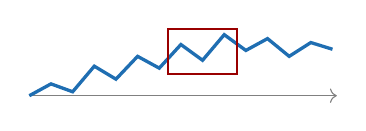
\begin{tikzpicture}[x=0.55cm,y=0.5cm]
  \draw[->,gray] (0,0)--(7.1,0);
  \draw[very thick,BootcampBlue] plot coordinates
    {(0,0)(.5,.3)(1,.1)(1.5,.75)(2,.42)(2.5,1)(3,.7)
     (3.5,1.3)(4,.9)(4.5,1.55)(5,1.15)(5.5,1.45)(6,1)(6.5,1.35)(7,1.18)};
  \draw[Crimson,thick] (3.2,.55) rectangle (4.8,1.7);
\end{tikzpicture}
\column{0.48\textwidth}
\centering\textbf{Zoomed segment}
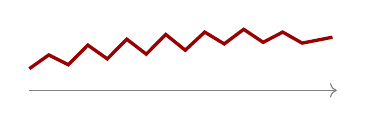
\begin{tikzpicture}[x=0.55cm,y=0.5cm]
  \draw[->,gray] (0,0)--(7.1,0);
  \draw[very thick,Crimson] plot coordinates
    {(0,.55)(.45,.9)(.9,.65)(1.35,1.15)(1.8,.8)(2.25,1.3)
     (2.7,.92)(3.15,1.42)(3.6,1.02)(4.05,1.48)(4.5,1.18)
     (4.95,1.55)(5.4,1.22)(5.85,1.48)(6.3,1.2)(7,1.35)};
\end{tikzpicture}
\end{columns}
Continuity means no jumps.
\begin{propositionblock}{Path roughness}
Almost surely, a Brownian path is nowhere differentiable and has infinite total variation on every nontrivial interval.
\end{propositionblock}
\textit{Heuristic:} the difference quotient has variance
\(\operatorname{Var}((W_{t+h}-W_t)/h)=1/h\), which explodes as \(h\downarrow0\).
\begin{block}{Bridge to quadratic variation}
Ordinary variation explodes, yet squared increments have a finite accumulated limit:
\([W]_t=t\). This is the roughness scale needed by stochastic calculus.
\end{block}
\end{frame}

\begin{frame}{Liminf and limsup quantify Brownian oscillations}
\footnotesize
\begin{propositionblock}{Perpetual oscillation}
Almost surely,
\[
\limsup_{t\to\infty}W_t=+\infty,
\qquad
\liminf_{t\to\infty}W_t=-\infty.
\]
Brownian motion therefore crosses every fixed level, positive or negative.
Nevertheless, on the linear scale,
\[
\liminf_{t\to+\infty}\frac{W_t}{t}
=\limsup_{t\to+\infty}\frac{W_t}{t}=0.
\]
For a two-sided Brownian motion, the same identities hold as $t\to-\infty$.
\end{propositionblock}
\begin{propositionblock}{Law of the iterated logarithm}
\[
\begin{aligned}
\limsup_{t\to\infty}\frac{W_t}{\sqrt{2t\log\log t}}&=1,
&\liminf_{t\to\infty}\frac{W_t}{\sqrt{2t\log\log t}}&=-1,\\
\limsup_{t\downarrow0}\frac{W_t}{\sqrt{2t\log\log(1/t)}}&=1,
&\liminf_{t\downarrow0}\frac{W_t}{\sqrt{2t\log\log(1/t)}}&=-1.
\end{aligned}
\]
\end{propositionblock}
\end{frame}

% =====================================================
\section{Markov Property as Renewal}
\subsection{Restarting at deterministic times}

\begin{frame}{The Markov idea separates past, present, and future}
\begin{center}
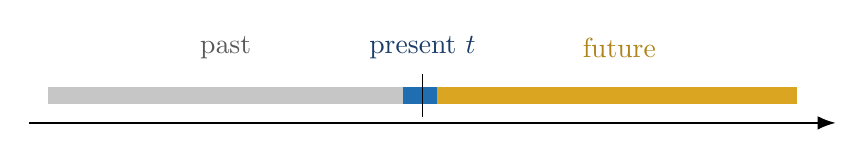
\begin{tikzpicture}[x=1.25cm,>=Latex]
  \draw[->,thick] (0,0)--(8.2,0);
  \draw[line width=6pt,gray!45] (.2,.35)--(3.8,.35);
  \draw[line width=6pt,BootcampBlue] (3.8,.35)--(4.15,.35);
  \draw[line width=6pt,AccentGold] (4.15,.35)--(7.8,.35);
  \node[gray!70!black] at (2,.95) {past};
  \node[BootcampBlueDark] at (4,.95) {present \(t\)};
  \node[AccentGold!80!black] at (6,.95) {future};
  \draw (4,.08)--(4,.62);
\end{tikzpicture}
\end{center}
\begin{definitionblock}{Markov principle, informal}
Given the present state, additional knowledge of the past does not improve the conditional law of the future.
\end{definitionblock}
The future is not independent of the present. The present is precisely the state that links past and future.
\end{frame}

\begin{frame}{At a fixed time, Brownian motion renews itself}
Fix \(t\ge0\) and define the future increments
\[
\widetilde W_u=W_{t+u}-W_t,
\qquad u\ge0.
\]
\begin{propositionblock}{Deterministic-time renewal}
\((\widetilde W_u)_{u\ge0}\) is a standard Brownian motion independent of \(\F_t\).
\end{propositionblock}
\textit{Proof idea:} \(\widetilde W_0=0\); its increments are Brownian increments after time \(t\), so they are independent of the past, Gaussian with variance equal to elapsed time, and stationary. Continuity is inherited from \(W\).
\begin{block}{Interpretation}
At time \(t\), retain the current level \(W_t\) and restart the noise from zero.
\end{block}
\end{frame}

\begin{frame}{The weak Markov property is a deterministic-time identity}
\begin{propositionblock}{Weak Markov property of Brownian motion}
For every bounded measurable function \(f\) and \(h\ge0\),
\[
\boxed{\E[f(W_{t+h})\mid\F_t]
=\E[f(W_{t+h})\mid W_t]
=(P_hf)(W_t)}.
\]
\end{propositionblock}
\textit{Proof.} Write
\[
W_{t+h}=W_t+\widetilde W_h,
\qquad \widetilde W_h\sim\mathcal N(0,h),
\qquad \widetilde W_h\perp\!\!\!\perp\F_t.
\]
Conditioning on \(\F_t\), only \(W_t\) remains random through the translation:
\[
(P_hf)(x)=\int_{\R}f(x+y)\frac{e^{-y^2/(2h)}}{\sqrt{2\pi h}}\,dy.
\]
\end{frame}

\begin{frame}{Weak Markov exercise: forecast from the current state}
At time \(2\), the whole path \((W_u)_{0\le u\le2}\) has been observed. On the branch where \(W_2=1\):
\begin{block}{Your turn -- 2 minutes}
Without using the detailed past path, compute
\begin{enumerate}\setlength{\itemsep}{0.6em}
  \item \(\Pp(W_5>2\mid W_2=1)\);
  \item \(\E[W_5^2\mid\F_2]\), then evaluate it when \(W_2=1\);
  \item the conditional law of \(W_5\) given \(\F_2\).
\end{enumerate}
\end{block}
\begin{block}{Diagnostic question}
Would knowing that the path crossed zero three times before time \(2\) change any answer once \(W_2\) is known?
\end{block}
\end{frame}

\begin{frame}{Weak Markov debrief: translate by the observed state}
Write
\[
W_5=W_2+(W_5-W_2)=W_2+\sqrt3\,Z,
\qquad Z\sim\mathcal N(0,1),\quad Z\perp\!\!\!\perp\F_2.
\]
Therefore
\[
W_5\mid\F_2\sim\mathcal N(W_2,3),
\qquad
\E[W_5^2\mid\F_2]=W_2^2+3.
\]
On the branch \(W_2=1\),
\[
\Pp(W_5>2\mid W_2=1)
=1-\Phi\!\left(\frac{1}{\sqrt3}\right)
\approx0.282,
\qquad
\E[W_5^2\mid W_2=1]=4.
\]
\begin{block}{Takeaway}
At a deterministic time, the present level is sufficient; the route taken to reach it is irrelevant for the future conditional law.
\end{block}
\end{frame}

\begin{frame}{Brownian motion is also a martingale}
For \(0\le s<t\),
\[
\E[W_t\mid\F_s]
=\E[W_s+(W_t-W_s)\mid\F_s]
=W_s.
\]
\begin{definitionblock}{Martingale interpretation}
Given all currently available information, the conditional expected future value equals the current value.
\end{definitionblock}
\begin{itemize}
  \item Markov: the current state summarizes the relevant past.
  \item Martingale: the current state is the best conditional mean forecast.
\end{itemize}
The two concepts are related here but are not synonymous.
\end{frame}

% =====================================================
\section{Stopping Times and Strong Markov Property}
\subsection{Stopping without looking ahead}

\begin{frame}{Discrete time makes the no-look-ahead rule visible}
Let \(\F_n=\sigma(X_0,\ldots,X_n)\) be the information observed by date \(n\).
\begin{definitionblock}{Discrete stopping time}
An integer-valued random time \(\tau\) is a stopping time if
\[
\{\tau\le n\}\in\F_n
\qquad\text{for every }n.
\]
\end{definitionblock}
\begin{columns}[T,onlytextwidth]
\column{0.48\textwidth}
\textbf{Observable: first hit}
\[
\tau_a=\inf\{n:X_n\ge a\}.
\]
At date \(n\), the observed path reveals whether a hit occurred.
\column{0.48\textwidth}
\textbf{Anticipative: last zero}
\[
\rho=\sup\{n\le N:X_n=0\}.
\]
Before \(N\), a later return to zero may still occur.
\end{columns}
\end{frame}

\begin{frame}{A stopping rule must be executable with information available now}
\begin{center}
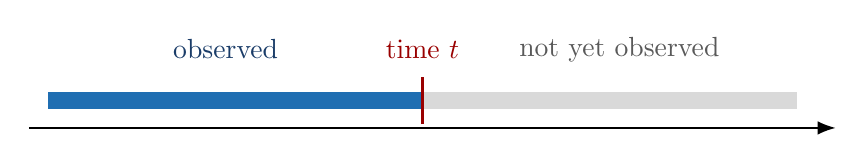
\begin{tikzpicture}[x=1.25cm,>=Latex]
  \draw[->,thick] (0,0)--(8.2,0);
  \draw[line width=6pt,BootcampBlue] (.2,.35)--(4,.35);
  \draw[line width=6pt,gray!30] (4,.35)--(7.8,.35);
  \draw[Crimson,very thick] (4,.05)--(4,.65);
  \node[BootcampBlueDark] at (2,1) {observed};
  \node[Crimson] at (4,1) {time \(t\)};
  \node[gray!70!black] at (6,1) {not yet observed};
\end{tikzpicture}
\end{center}
\begin{block}{Operational question}
At time \(t\), can I determine whether the rule has already triggered?
\end{block}
\begin{itemize}
  \item If yes for every \(t\), the random time is admissible.
  \item If the answer requires seeing the future path, it is not.
\end{itemize}
\end{frame}

\begin{frame}{The definition turns the operational question into measurability}
Let \((\F_t)_{t\ge0}\) represent the information observed through time.
\begin{definitionblock}{Stopping time}
A random time \(\tau:\Omega\to[0,\infty]\) is a stopping time if
\[
\{\tau\le t\}\in\F_t
\qquad\text{for every }t\ge0.
\]
\end{definitionblock}
The event \(\{\tau\le t\}\) means "the rule has triggered by time \(t\)." It must be answerable using only information in \(\F_t\).
\begin{block}{Important distinction}
A stopping time is random, but it is not anticipative.
\end{block}
\end{frame}

\begin{frame}{Deterministic times and first hitting times are stopping times}
\begin{columns}[T,onlytextwidth]
\column{0.48\textwidth}
\begin{definitionblock}{Deterministic time}
For \(\tau=t_0\),
\[
\{\tau\le t\}=
\begin{cases}
\emptyset,&t<t_0,\\
\Omega,&t\ge t_0.
\end{cases}
\]
\end{definitionblock}
\column{0.48\textwidth}
\begin{definitionblock}{First hit of level \(a\)}
\[
\tau_a=\inf\{t\ge0:W_t=a\}.
\]
By continuity,
\[
\{\tau_a\le t\}
=\left\{\max_{0\le u\le t}W_u\ge a\right\}\in\F_t
\]
for \(a>0\).
\end{definitionblock}
\end{columns}
Both rules can be verified as the path unfolds.
\end{frame}

\begin{frame}{First exit from an interval uses only the observed path}
For \(\ell<u\), define
\[
\tau_{\ell,u}=\inf\{t\ge0:W_t\notin(\ell,u)\}.
\]
\begin{center}
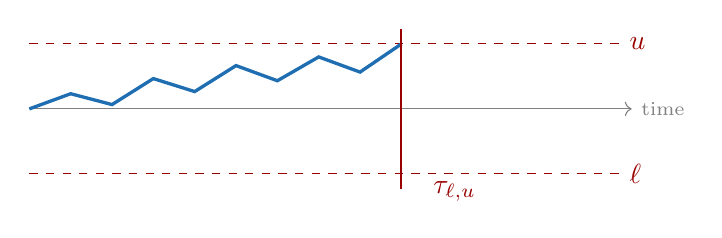
\begin{tikzpicture}[x=.75cm,y=.55cm]
  \draw[->,gray] (0,0)--(10.2,0) node[right] {\scriptsize time};
  \draw[dashed,Crimson] (0,1.5)--(10,1.5) node[right] {\(u\)};
  \draw[dashed,Crimson] (0,-1.5)--(10,-1.5) node[right] {\(\ell\)};
  \draw[very thick,BootcampBlue] plot coordinates
    {(0,0)(.7,.35)(1.4,.1)(2.1,.7)(2.8,.4)(3.5,1)
     (4.2,.65)(4.9,1.2)(5.6,.85)(6.3,1.5)};
  \draw[Crimson,thick] (6.3,-1.85)--(6.3,1.85);
  \node[Crimson] at (7.2,-1.9) {\(\tau_{\ell,u}\)};
\end{tikzpicture}
\end{center}
By time \(t\), we know whether the observed path has left the interval. No future information is needed.
\end{frame}

\begin{frame}{The last zero before a horizon is not a stopping time}
Fix \(T>0\) and define
\[
\rho=\sup\{0\le u\le T:W_u=0\}.
\]
\begin{center}
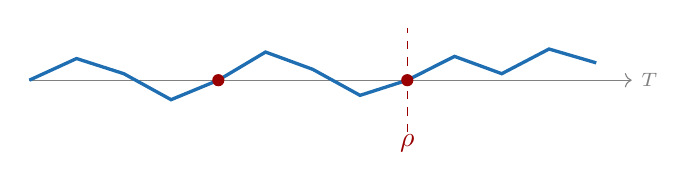
\begin{tikzpicture}[x=.75cm,y=.55cm]
  \draw[->,gray] (0,0)--(10.2,0) node[right] {\scriptsize \(T\)};
  \draw[very thick,BootcampBlue] plot coordinates
    {(0,0)(.8,.5)(1.6,.15)(2.4,-.45)(3.2,0)(4,.65)
     (4.8,.25)(5.6,-.35)(6.4,0)(7.2,.55)(8,.15)(8.8,.72)(9.6,.4)};
  \fill[Crimson] (3.2,0) circle (2.2pt);
  \fill[Crimson] (6.4,0) circle (2.2pt);
  \draw[dashed,Crimson] (6.4,-1.2)--(6.4,1.2);
  \node[Crimson] at (6.4,-1.45) {\(\rho\)};
\end{tikzpicture}
\end{center}
When the path is at zero at time \(t<T\), we cannot know whether it will return to zero later. Identifying the \emph{last} zero requires the future path.
\end{frame}

\begin{frame}{Quick check: which random times are stopping times?}
Fix \(T>0\). Consider:
\begin{enumerate}\setlength{\itemsep}{0.55em}
  \item \(\tau_1=\inf\{t\ge0:W_t\ge1\}\);
  \item \(\tau_2=T/2\);
  \item \(\tau_3=\inf\{t\ge T/2:W_t=0\}\);
  \item \(\tau_4=\operatorname*{arg\,max}_{0\le t\le T}W_t\).
\end{enumerate}
\pause
\begin{block}{Answer}
\(\tau_1,\tau_2,\tau_3\) are stopping times. The time \(\tau_4\) of the maximum is not: deciding that the current value is the maximum requires observing the rest of the path.
\end{block}
\end{frame}

\subsection{Strong Markov property}

\begin{frame}{\(\F_\tau\) is the information available when the rule triggers}
\begin{definitionblock}{Stopped sigma-field}
For a stopping time \(\tau\), define
\[
\F_\tau
=\bigl\{A\in\F:\ A\cap\{\tau\le t\}\in\F_t
\text{ for every }t\ge0\bigr\}.
\]
\end{definitionblock}
An event in \(\F_\tau\) can be decided using only the information revealed by the random time \(\tau\).
\begin{block}{Discrete-time picture}
If \(\tau\) takes integer values, then
\(A\in\F_\tau\) iff \(A\cap\{\tau=n\}\in\F_n\) for every \(n\).
On each branch \(\{\tau=n\}\), only observations through date \(n\) may be used.
\end{block}
\end{frame}

\begin{frame}{Strong Markov means that Brownian motion restarts at a stopping time}
Let \(\tau\) be an almost surely finite stopping time. Then
\[
\widetilde W_u=W_{\tau+u}-W_\tau,\qquad u\ge0,
\]
is a Brownian motion independent of the information \(\F_\tau\) available when stopping.
\begin{center}
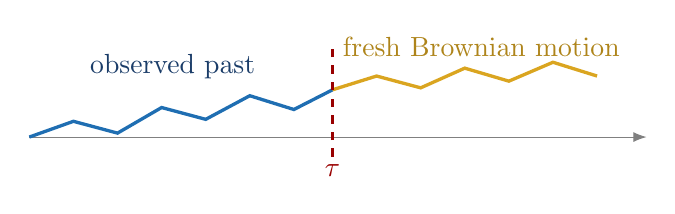
\begin{tikzpicture}[x=.7cm,y=.5cm,>=Latex]
  \draw[->,gray] (0,0)--(11.2,0);
  \draw[very thick,BootcampBlue] plot coordinates
   {(0,0)(.8,.4)(1.6,.1)(2.4,.75)(3.2,.45)(4,1.05)(4.8,.7)(5.5,1.2)};
  \draw[very thick,AccentGold] plot coordinates
   {(5.5,1.2)(6.3,1.55)(7.1,1.25)(7.9,1.75)(8.7,1.42)(9.5,1.9)(10.3,1.55)};
  \draw[dashed,Crimson,thick] (5.5,-.5)--(5.5,2.3);
  \node[Crimson] at (5.5,-.85) {\(\tau\)};
  \node[BootcampBlueDark] at (2.6,1.8) {observed past};
  \node[AccentGold!80!black] at (8.2,2.3) {fresh Brownian motion};
\end{tikzpicture}
\end{center}
\small Ordinary Markov restarts at a fixed time; strong Markov restarts when an observable event occurs.
\end{frame}

\begin{frame}{Strong Markov exercise: restart when a barrier is reached}
Let
\[
\tau_1=\inf\{t\ge0:W_t=1\}.
\]
Brownian motion reaches level \(1\) almost surely, so \(W_{\tau_1}=1\).
\begin{block}{Your turn -- 3 minutes}
Use strong Markov to answer:
\begin{enumerate}\setlength{\itemsep}{0.55em}
  \item What is the conditional law of \(W_{\tau_1+h}\) given \(\F_{\tau_1}\)?
  \item Compute \(\Pp(W_{\tau_1+2}\ge2\mid\F_{\tau_1})\).
  \item If \(\rho=\inf\{u\ge0:W_{\tau_1+u}=3\}\), which familiar first-passage time has the same law as \(\rho\)?
\end{enumerate}
\end{block}
The key is to recenter both time and space at the random point \((\tau_1,1)\).
\end{frame}

\begin{frame}{Strong Markov debrief: the post-hit increment is fresh}
\small
Define \(B_h=W_{\tau_1+h}-W_{\tau_1}\). Strong Markov gives
\[
(B_h)_{h\ge0}\text{ is Brownian and independent of }\F_{\tau_1}.
\]
Hence
\[
W_{\tau_1+h}\mid\F_{\tau_1}\sim\mathcal N(1,h)
\]
and
\[
\Pp(W_{\tau_1+2}\ge2\mid\F_{\tau_1})
=1-\Phi\!\left(\frac1{\sqrt2}\right)
\approx0.240.
\]
To reach level \(3\) after \(\tau_1\), the fresh Brownian motion \(B\) must travel from \(0\) to \(2\). Therefore
\[
\rho\ \overset d=\ \tau_2.
\]
\begin{block}{Contrast}
Weak Markov restarts at a fixed clock time; strong Markov restarts at an observable random time.
\end{block}
\end{frame}

\begin{frame}{Strong Markov is the bridge from stopping to reflection}
Suppose a Brownian path first hits level \(a>0\) at
\[
\tau_a=\inf\{u\ge0:W_u=a\}.
\]
After \(\tau_a\),
\[
W_{\tau_a+u}-a
\]
is a fresh Brownian motion, independent of how the path reached \(a\).
\begin{block}{Why this matters}
Because a fresh Brownian motion is symmetric, we may flip the sign of every increment after \(\tau_a\) without changing its law.
\end{block}
That sign flip is exactly the reflection principle.
\end{frame}

% =====================================================
\section{Reflection Principle and Hitting Probabilities}
\subsection{Path transformation}

\begin{frame}{Step 1: stop at the first barrier hit}
Let \(a>0\) and \(\tau_a=\inf\{u\ge0:W_u=a\}\).
\begin{center}
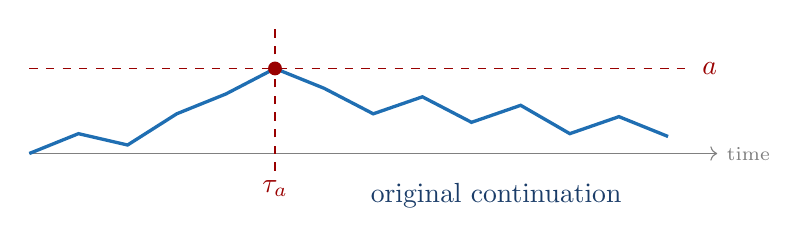
\begin{tikzpicture}[x=.78cm,y=.72cm]
  \draw[->,gray] (0,0)--(11.2,0) node[right] {\scriptsize time};
  \draw[dashed,Crimson] (0,1.5)--(10.8,1.5) node[right] {\(a\)};
  \draw[very thick,BootcampBlue] plot coordinates
    {(0,0)(.8,.35)(1.6,.15)(2.4,.7)(3.2,1.05)(4,1.5)
     (4.8,1.15)(5.6,.7)(6.4,1)(7.2,.55)(8,.85)(8.8,.35)(9.6,.65)(10.4,.3)};
  \draw[dashed,Crimson,thick] (4,-.3)--(4,2.2);
  \fill[Crimson] (4,1.5) circle (2.5pt);
  \node[Crimson] at (4,-.62) {\(\tau_a\)};
  \node[BootcampBlueDark] at (7.6,-.75) {original continuation};
\end{tikzpicture}
\end{center}
The first part of the path identifies when reflection starts. Only the continuation after \(\tau_a\) will change.
\end{frame}

\begin{frame}{Step 2: reflect only the fresh continuation}
For a path that hits \(a\), define
\[
W_u^\star=
\begin{cases}
W_u,&u\le\tau_a,\\
2a-W_u,&u>\tau_a.
\end{cases}
\]
\begin{center}
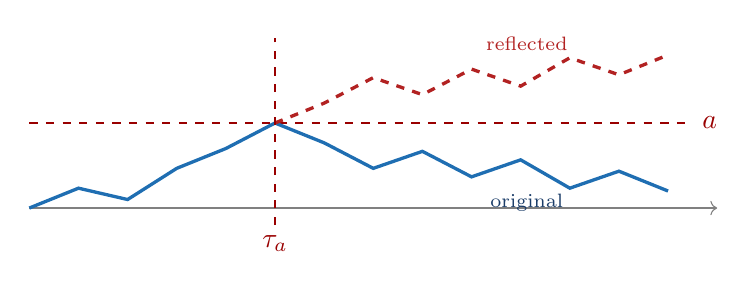
\begin{tikzpicture}[x=.78cm,y=.72cm]
  \draw[->,gray] (0,0)--(11.2,0);
  \draw[dashed,Crimson] (0,1.5)--(10.8,1.5) node[right] {\(a\)};
  \draw[very thick,BootcampBlue] plot coordinates
    {(0,0)(.8,.35)(1.6,.15)(2.4,.7)(3.2,1.05)(4,1.5)};
  \draw[very thick,BootcampBlue] plot coordinates
    {(4,1.5)(4.8,1.15)(5.6,.7)(6.4,1)(7.2,.55)(8,.85)(8.8,.35)(9.6,.65)(10.4,.3)};
  \draw[very thick,MatrixRed,dashed] plot coordinates
    {(4,1.5)(4.8,1.85)(5.6,2.3)(6.4,2)(7.2,2.45)(8,2.15)(8.8,2.65)(9.6,2.35)(10.4,2.7)};
  \draw[dashed,Crimson,thick] (4,-.3)--(4,3);
  \node[Crimson] at (4,-.62) {\(\tau_a\)};
  \node[BootcampBlueDark] at (8.1,.1) {\scriptsize original};
  \node[MatrixRed] at (8.1,2.9) {\scriptsize reflected};
\end{tikzpicture}
\end{center}
Strong Markov plus symmetry implies that the reflected path has the same Brownian probability law.
\end{frame}

\begin{frame}{Step 3: pair terminal events path by path}
Let
\[
M_t=\max_{0\le u\le t}W_u.
\]
Among paths that reach \(a\) before \(t\), reflection gives a one-to-one correspondence:
\[
\{M_t\ge a,\ W_t<a\}
\quad\longleftrightarrow\quad
\{W_t>a\}.
\]
\begin{center}
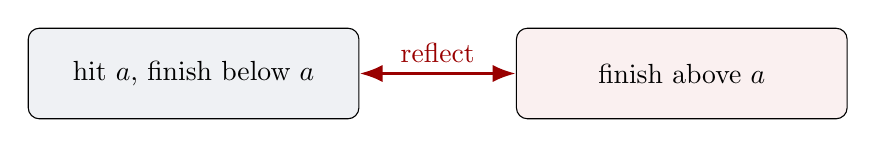
\begin{tikzpicture}[>=Latex]
  \node[draw,rounded corners,fill=BootcampBlueDark!7,
        minimum width=4.2cm,minimum height=1.15cm] (l) at (0,0)
        {hit \(a\), finish below \(a\)};
  \node[draw,rounded corners,fill=MatrixRed!7,
        minimum width=4.2cm,minimum height=1.15cm] (r) at (6.2,0)
        {finish above \(a\)};
  \draw[<->,very thick,Crimson] (l)--(r) node[midway,above] {reflect};
\end{tikzpicture}
\end{center}
The equality of probabilities follows from this measure-preserving pairing.
\end{frame}

\subsection{Consequences}

\begin{frame}{Theorem: reflection doubles a Gaussian tail}
The event \(\{M_t\ge a\}\) splits into two disjoint cases:
\[
\{M_t\ge a\}
=\{W_t\ge a\}
\cup
\{M_t\ge a,\ W_t<a\}.
\]
Reflection gives
\[
\Pp(M_t\ge a,\ W_t<a)=\Pp(W_t>a).
\]
Since \(\Pp(W_t=a)=0\),
\[
\boxed{\Pp(M_t\ge a)=2\Pp(W_t\ge a)}
=2\left(1-\Phi\!\left(\frac{a}{\sqrt t}\right)\right).
\]
The running maximum has the same one-dimensional distribution as \(|W_t|\).
\end{frame}

\begin{frame}{Corollary: first-passage times have an explicit law}
For \(\tau_a=\inf\{u\ge0:W_u=a\}\),
\[
\{\tau_a\le t\}=\{M_t\ge a\}.
\]
Therefore
\[
\boxed{\Pp(\tau_a\le t)
=2\left(1-\Phi\!\left(\frac{a}{\sqrt t}\right)\right)}.
\]
Differentiating yields
\[
f_{\tau_a}(t)
=\frac{a}{\sqrt{2\pi t^3}}
\exp\!\left(-\frac{a^2}{2t}\right),
\qquad t>0.
\]
Thus Brownian motion eventually reaches every fixed level \(a\) with probability one.
\end{frame}

\begin{frame}{Application: a four-year barrier probability}
What is the probability that Brownian motion reaches level \(1\) before time \(4\)?

Since \(\{\tau_1\le4\}=\{M_4\ge1\}\), the reflection principle gives
\[
\Pp(\tau_1\le4)
=2\left(1-\Phi\!\left(\frac{1}{\sqrt4}\right)\right)
=2\bigl(1-\Phi(0.5)\bigr)
\approx0.617.
\]

\begin{block}{Interpretation}
Although \(W_4\sim\mathcal N(0,4)\), the barrier event depends on the whole path, not only on the terminal value. Reflection converts that path-dependent event into a Gaussian tail.
\end{block}
\end{frame}

\begin{frame}{Finance application: a barrier claim is a first-passage problem}
\small
Under the risk-neutral measure,
\[
S_t=S_0\exp\!\left(\nu t+\sigma W_t\right),
\qquad
\nu=r-\tfrac12\sigma^2.
\]
For an upper barrier \(H>S_0\), define
\(\tau_H=\inf\{t:S_t\ge H\}\) and \(a=\log(H/S_0)\). Then
\[
\{\tau_H\le T\}
=\left\{\max_{0\le t\le T}(\nu t+\sigma W_t)\ge a\right\}.
\]
\begin{propositionblock}{Zero log-drift case \(\nu=0\)}
The ordinary reflection principle gives
\[
\boxed{\Pp(\tau_H\le T)
=2\left[1-\Phi\!\left(\frac{\log(H/S_0)}{\sigma\sqrt T}\right)\right].}
\]
\end{propositionblock}
With nonzero \(\nu\), the drifted reflection formula adds an exponential tilt.
\end{frame}

\begin{frame}{Worked finance example: value a one-touch digital}
\small
Consider a one-year contract with
\[
S_0=100,\qquad H=120,\qquad T=1,\qquad
r=2\%,\qquad \sigma=20\%.
\]
Here \(\nu=r-\tfrac12\sigma^2=0\), and therefore
\[
a=\log(1.2)\approx0.1823,
\qquad
\frac{a}{\sigma\sqrt T}\approx0.9116.
\]
Reflection gives the probability of touching \(120\) before maturity:
\[
\Pp(\tau_{120}\le1)
=2\bigl[1-\Phi(0.9116)\bigr]
\approx0.362.
\]
A claim paying one dollar at \(T\) after a touch is worth
\[
V_0=e^{-rT}\Pp(\tau_{120}\le1)
\approx e^{-0.02}(0.362)
\approx0.355.
\]
\medskip
\textbf{Financial interpretation.}
Reflection turns continuous monitoring into a Gaussian-tail calculation and underlies barrier-option formulas.
\end{frame}

% =====================================================
\section{Quadratic Variation and Brownian Roughness}
\subsection{Why ordinary calculus is not enough}

\begin{frame}{Non-differentiability suggests a different notion of variation}
On a partition \(0=t_0<\cdots<t_n=T\), write
\[
\Delta_iW=W_{t_{i+1}}-W_{t_i}.
\]
For an evenly spaced grid, \(\Delta_iW\) typically has size \(\sqrt{T/n}\). Thus
\[
\sum_{i=0}^{n-1}(\Delta_iW)^2
\quad\text{has typical size}\quad
n\times\frac{T}{n}=T.
\]
\begin{block}{Contrast with smooth paths}
For a differentiable path, increments have size \(T/n\), so the sum of squared increments has size \(n(T/n)^2\to0\).
\end{block}
Brownian paths have infinite ordinary variation, but their squared increments accumulate to a finite limit. This is the useful replacement for a nonexistent derivative.
\end{frame}

\begin{frame}{Quadratic variation records accumulated squared increments}
For a continuous process \(X\) and partitions
\[
\pi_n=\{0=t_0^n<\cdots<t_{k_n}^n=t\},
\qquad |\pi_n|\to0,
\]
define
\[
[X]_t
=\lim_{n\to\infty}
\sum_i\left(X_{t_{i+1}^n}-X_{t_i^n}\right)^2,
\]
when the limit exists in probability.
\begin{definitionblock}{Interpretation}
\([X]_t\) measures the amount of fine-scale path fluctuation accumulated up to time \(t\).
\end{definitionblock}
\end{frame}

\begin{frame}{Quadratic variation is itself an accumulated-variation process}
When it exists, \(([X]_t)_{t\ge0}\) starts at zero and is nondecreasing. It measures fluctuation, not the direction of moves.
\begin{propositionblock}{Elementary properties}
If \(A\) is continuous with finite variation, then
\[
[A]_t=0,
\qquad
[X+A]_t=[X]_t,
\qquad
[aX]_t=a^2[X]_t.
\]
\end{propositionblock}
\textit{Proof idea:} fine increments of \(A\) are uniformly small, while their absolute sum remains bounded; hence their squared sum and cross-term with \(X\) vanish.
\begin{block}{Numerical meaning}
On a fine observation grid, the realized sum \(\sum_i(\Delta_iX)^2\) estimates the accumulated quadratic variation.
\end{block}
\end{frame}

\begin{frame}{Smooth paths have zero quadratic variation}
Let \(x\) be continuously differentiable on \([0,T]\). By the mean value theorem,
\[
x_{t_{i+1}}-x_{t_i}=x'(\xi_i)(t_{i+1}-t_i).
\]
Hence
\[
\sum_i(x_{t_{i+1}}-x_{t_i})^2
\le
\|x'\|_\infty^2
|\pi_n|\sum_i(t_{i+1}-t_i)
=\|x'\|_\infty^2T|\pi_n|\to0.
\]
\begin{block}{Example}
For \(x_t=t\), an equal grid gives \(n(T/n)^2=T^2/n\to0\).
\end{block}
\end{frame}

\begin{frame}{Brownian motion has quadratic variation equal to elapsed time}
\begin{definitionblock}{Fundamental result}
For Brownian motion and any fixed \(t\ge0\),
\[
\boxed{[W]_t=t}
\]
in probability along partitions whose mesh tends to zero.
\end{definitionblock}
On an equal grid with \(\Delta t=t/n\),
\[
\E\!\left[\sum_{i=0}^{n-1}(\Delta_iW)^2\right]
=\sum_{i=0}^{n-1}\E[(\Delta_iW)^2]
=n\Delta t=t.
\]
The randomness of the sum vanishes as the grid is refined.
\end{frame}

\begin{frame}{A short variance calculation explains concentration around \(t\)}
For independent \(\Delta_iW\sim\mathcal N(0,\Delta t)\),
\[
\operatorname{Var}\!\left((\Delta_iW)^2\right)=2(\Delta t)^2.
\]
Therefore
\[
\operatorname{Var}\!\left(
\sum_{i=0}^{n-1}(\Delta_iW)^2
\right)
=2n(\Delta t)^2
=\frac{2t^2}{n}\longrightarrow0.
\]
Thus the sum of squared increments converges to \(t\) in \(L^2\), hence in probability.
\begin{block}{Meaning}
Each squared increment is random, but their accumulated total becomes deterministic.
\end{block}
\end{frame}

\begin{frame}{What \([X]_t\) tells us about a process}
\begin{center}
\begin{tabular}{lll}
\toprule
Process & Quadratic variation & What survives at fine scale \\
\midrule
smooth or finite-variation \(A\) & \([A]_t=0\) & no rough component \\
Brownian motion \(W\) & \([W]_t=t\) & one variance unit per time unit \\
\(X_t=A_t+\sigma W_t\) & \([X]_t=\sigma^2t\) & volatility, not drift \\
\bottomrule
\end{tabular}
\end{center}
\begin{block}{Key message}
Quadratic variation is a pathwise record of accumulated volatility. It ignores smooth drift and retains persistent small-scale randomness.
\end{block}
This is why high-frequency squared returns are the starting point for realized-volatility estimation.
\end{frame}

\begin{frame}{The bracket corrects the square of a martingale}
\begin{propositionblock}{Quadratic-variation martingale}
For a continuous square-integrable martingale \(X\), there is a unique increasing predictable process \(\langle X\rangle\), starting from zero, such that
\[
\boxed{X_t^2-\langle X\rangle_t\text{ is a martingale}.}
\]
For continuous martingales, \(\langle X\rangle=[X]\).
\end{propositionblock}
For Brownian motion, \(\langle W\rangle_t=[W]_t=t\). Since
\[
\E[W_t^2\mid\F_s]=W_s^2+(t-s).
\]
we obtain
\[
\E[W_t^2-t\mid\F_s]=W_s^2-s.
\]
Hence \(W_t^2-t\) is a martingale.
\end{frame}

\begin{frame}{The It\^o multiplication table summarizes the new calculus}
Brownian scaling suggests \(dW_t\) has size \(\sqrt{dt}\). Hence
\[
(dW_t)^2=dt,
\qquad
dW_t\,dt=0,
\qquad
(dt)^2=0.
\]
\begin{center}
\begin{tabular}{c|cc}
\toprule
\(\times\) & \(dt\) & \(dW_t\)\\
\midrule
\(dt\) & \(0\) & \(0\)\\
\(dW_t\) & \(0\) & \(dt\)\\
\bottomrule
\end{tabular}
\end{center}
\begin{block}{Preview}
The identity \((dW_t)^2=dt\) is why It\^o's formula contains a second-derivative term.
\end{block}
\end{frame}

\begin{frame}{Discrete trading gains lead naturally to stochastic integrals}
On a trading grid,
\[
G_T^{(n)}
=\sum_{i=0}^{n-1}\Delta_{t_i}
\bigl(S_{t_{i+1}}-S_{t_i}\bigr),
\]
where \(\Delta_{t_i}\) is chosen using information available at \(t_i\).
As the mesh tends to zero, the limiting gain is written
\[
G_T=\int_0^T\Delta_t\,dS_t.
\]
\begin{itemize}
  \item Adaptedness prevents look-ahead trading.
  \item Quadratic variation determines the calculus of the limit.
  \item The next lectures make this construction and It\^o's formula precise.
\end{itemize}
\end{frame}

% =====================================================
\section{From Brownian Motion to a Positive Price Model}
\subsection{Geometric Brownian motion}

\begin{frame}{An additive Brownian price can become negative}
The model
\[
S_t=S_0+\mu t+\sigma W_t
\]
has Gaussian values with support on all of \(\R\).
\begin{columns}[T,onlytextwidth]
\column{0.52\textwidth}
\begin{itemize}
  \item Negative prices are possible.
  \item Absolute volatility is constant, regardless of the price level.
  \item Financial returns are usually modeled multiplicatively instead.
\end{itemize}
\column{0.43\textwidth}
\centering
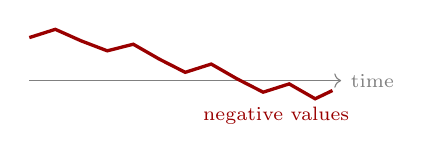
\begin{tikzpicture}[x=.55cm,y=.42cm]
  \draw[->,gray] (0,0)--(7.2,0) node[right] {\scriptsize time};
  \draw[very thick,Crimson] plot coordinates
   {(0,1.3)(.6,1.55)(1.2,1.2)(1.8,.9)(2.4,1.1)(3,.65)
    (3.6,.25)(4.2,.5)(4.8,.05)(5.4,-.35)(6,-.1)(6.6,-.55)(7,-.3)};
  \node[Crimson] at (5.7,-1.05) {\scriptsize negative values};
\end{tikzpicture}
\end{columns}
\end{frame}

\begin{frame}{Exponentiating Brownian log-returns keeps prices positive}
Assume the log-price follows
\[
\log\frac{S_t}{S_0}
=\left(\mu-\frac12\sigma^2\right)t+\sigma W_t.
\]
Then
\[
\boxed{
S_t=S_0
\exp\!\left(
\left(\mu-\frac12\sigma^2\right)t+\sigma W_t
\right)}
\]
is a geometric Brownian motion.
\begin{itemize}
  \item \(S_t>0\) for every \(t\).
  \item Log-returns over disjoint intervals are independent.
  \item Their variance is proportional to elapsed time.
\end{itemize}
\end{frame}

\begin{frame}{Worked example: one-year distribution under GBM}
Let
\[
S_0=100,
\qquad \mu=8\%,
\qquad \sigma=20\%,
\qquad t=1.
\]
Then
\[
\log\frac{S_1}{100}
\sim\mathcal N(0.08-\tfrac12(0.20)^2,\,(0.20)^2)
=\mathcal N(0.06,0.04).
\]

Therefore
\[
\operatorname{Median}(S_1)=100e^{0.06}\approx106.18,
\qquad
\E[S_1]=100e^{0.08}\approx108.33.
\]

The mean exceeds the median because a lognormal distribution is right-skewed.
\end{frame}

\begin{frame}{The drift controls the mean; volatility controls dispersion}
For geometric Brownian motion,
\[
\E[S_t]=S_0e^{\mu t},
\qquad
\operatorname{Var}(S_t)
=S_0^2e^{2\mu t}\bigl(e^{\sigma^2t}-1\bigr).
\]
Over a short interval \(\Delta t\),
\[
\log\frac{S_{t+\Delta t}}{S_t}
\approx\mathcal N\!\left(
\left(\mu-\tfrac12\sigma^2\right)\Delta t,\,
\sigma^2\Delta t
\right).
\]
\begin{block}{Square-root-of-time rule}
The standard deviation of a log-return over \(\Delta t\) is \(\sigma\sqrt{\Delta t}\).
\end{block}
\end{frame}

\begin{frame}{Quadratic variation identifies accumulated log-price volatility}
Let
\[
X_t=\log S_t
=\log S_0+\left(\mu-\tfrac12\sigma^2\right)t+\sigma W_t.
\]
The finite-variation drift has zero quadratic variation, so
\[
\boxed{[X]_t=\sigma^2[W]_t=\sigma^2t.}
\]
\begin{block}{Interpretation}
Quadratic variation filters out the smooth drift and retains the cumulative variance generated by Brownian shocks.
\end{block}
This connection underlies realized-volatility estimators based on high-frequency squared returns.
\end{frame}

\begin{frame}{GBM is useful, but its assumptions are visible}
\begin{columns}[T,onlytextwidth]
\column{0.47\textwidth}
\textbf{What it captures}
\begin{itemize}
  \item positive prices;
  \item random continuous returns;
  \item explicit conditional laws;
  \item a tractable volatility parameter.
\end{itemize}
\column{0.47\textwidth}
\textbf{What it misses}
\begin{itemize}
  \item jumps and extreme tails;
  \item changing volatility;
  \item volatility smiles;
  \item long-range market effects.
\end{itemize}
\end{columns}
\begin{block}{Modeling lesson}
Brownian motion is a foundational building block, not a complete description of every market feature.
\end{block}
\end{frame}

\end{document}
